% ======================================================================
%
% Copyright (c) 1999 The GALIA Consortium
%
% This software and related documentation is part of the
% Computational Geometry Algorithms Library (CGAL).
%
% Every use of CGAL requires a license. Licenses come in three kinds:
%
% - For academic research and teaching purposes, permission to use and
%   copy the software and its documentation is hereby granted free of  
%   charge, provided that
%   (1) it is not a component of a commercial product, and
%   (2) this notice appears in all copies of the software and
%       related documentation.
% - Development licenses grant access to the source code of the library 
%   to develop programs. These programs may be sold to other parties as 
%   executable code. To obtain a development license, please contact
%   the GALIA Consortium (at cgal@cs.uu.nl).
% - Commercialization licenses grant access to the source code and the
%   right to sell development licenses. To obtain a commercialization 
%   license, please contact the GALIA Consortium (at cgal@cs.uu.nl).
%
% This software and documentation is provided "as-is" and without
% warranty of any kind. In no event shall the CGAL Consortium be
% liable for any damage of any kind.
%
% The GALIA Consortium consists of Utrecht University (The Netherlands),
% ETH Zurich (Switzerland), Free University of Berlin (Germany),
% INRIA Sophia-Antipolis (France), Martin-Luther-University Halle-Wittenberg
% (Germany), Max-Planck-Institute Saarbrucken (Germany),
% and Tel-Aviv University (Israel).
%
% ----------------------------------------------------------------------
%
% package       : Alpha_shapes_2
% author(s)     : Tran Kai Frank DA <Frank.Da@sophia.inria.fr>
%
% coordinator   : INRIA Sophia-Antipolis (<Mariette.Yvinec@sophia.inria.fr>)
%
% ======================================================================

\RCSdef{\alphashapeRevision}{$Revision$}
\RCSdefDate{\alphashapeDate}{$Date$}

%----------------------------------------------------------------------

\chapter{2D Alpha Shapes} \label{I1_ChapterAlphashapes2D}

%\ccChapterSubTitle{\alphashapeRevision, \alphashapeDate}
\begin{ccTexOnly}
\vspace*{-1cm}
\includegraphics{alphashape.eps} 
\end{ccTexOnly}
\begin{ccHtmlOnly}
<img border=0 src="./alphashape.gif"  align=center>
\end{ccHtmlOnly}

Assume we are given a set $S$ of points in 2D or 3D and we'd like to
have something like ``the shape formed by these points.'' This is
quite a vague notion and there are probably many possible
interpretations, the $\alpha$-shape being one of them. Alpha shapes
can be used for shape reconstruction from a dense unorganized set of
data points. Indeed, an $\alpha$-shape is demarcated by a frontier,
which is a linear approximation of the original contour \cite{bb-srmua-97t}.

As mentionned in Edelsbrunner's and M\"ucke's paper \cite{em-tdas-94},
one can intuitively think of an $\alpha$-shape as the
following. Imagine a huge mass of ice-cream making up the space $\R^3$
and containing the points as ``hard'' chocolate pieces. Using one of
these sphere-formed ice-cream spoons we carve out all parts of the
ice-cream block we can reach without bumping into chocolate pieces,
thereby even carving out holes in the inside (eg. parts not reachable
by simply moving the spoon from the outside). We will eventually end
up with a (not necessarily convex) object bounded by caps, arcs and
points. If we now straighten all ``round'' faces to triangles and line
segments, we have an intuitive description of what is called the
$\alpha$-shape of $S$. Here's an example for this process in 2D (where
our ice-cream spoon is simply a circle):
                                                                        
And what is $\alpha$ in the game?  $\alpha$ is the radius of the
carving spoon. A very small value will allow us to eat up all of the
ice-cream except the chocolate points themselves. Thus we already see
that the $\alpha$-shape of degenerates to the point-set $S$ for
$\alpha \rightarrow 0$. On the other hand, a huge value of $\alpha$
will prevent us even from moving the spoon between two points since
it's way too large. So we will never spoon up ice-cream lying in the
inside of the convex hull of $S$, and hence the $\alpha$-shape for
$\alpha \rightarrow \infty$ is the convex hull of $S$.\footnote{ice cream, ice cream!!!
The wording of this introductory paragraphs is borrowed from  Kaspar Fischer's
`` Introduction to Alpha Shapes'' which can be found at 
http://n.ethz.ch/student/fischerk/alphashapes/as/index.html.
The picture has been taken from Walter Luh's homepage at
http://www.stanford.edu/~wluh/cs448b/alphashapes.html.}


\section{Definitions}

% Alpha shapes are the generalization of the convex hull of a point
% set. Let $S$ be a finite set of points in $\R^d$, $d = 2,3$ and
% $\alpha$ a parameter with $0 \leq \alpha \leq
% \infty$. For $\alpha = \infty$, the $\alpha$-shape is the convex hull of $S$. As 
% $\alpha$ decreases, the $\alpha$-shape shrinks and develops cavities,
% as soon as a sphere of radius $\sqrt{\alpha}$ can be put inside.
% Finally, for $\alpha = 0$, the $\alpha$-shape is the set $S$ itself.

We distinguish two versions of alpha shapes.  {\em Basic alpha shapes}
are based on the Delaunay triangulation.  {\em Weighted alpha shapes}
are based on its generalization, the regular triangulation, replacing
the natural distance by the power to weighted points. 

% The {\em basic alpha shapes} (cf. \ref{I1_SectClassicAS2D}) associated
% with the Delaunay triangulations (cf. \ref{I1_Sect_Delaunay}), in the
% other hand, the {\em weighted alpha shapes}
% (cf. \ref{I1_SectWeightedAS2D}) associated with the regular
% triangulations (cf. \ref{I1_Sect_Regular}).

There is a close connection between alpha shapes and the underlying
triangulations. More precisely, the $\alpha$-complex of $S$ is a
subcomplex of this triangulation of $S$, containing the $\alpha$-exposed
$k$-simplices, $0 \leq k \leq d$. A simplex is $\alpha$-exposed, if there is an
open disk (resp.\ ball) of radius $\sqrt{\alpha}$ through the vertices of the
simplex that does not contain any other point of $S$, for the metric used in
the computation of the underlying triangulation.  The corresponding
$\alpha$-shape is defined as the underlying interior space of the
$\alpha$-complex. 

In general, an $\alpha$-complex is a non-connected and non-pure polytope, it
means, that one $k$-simplex, $0 \leq k \leq d-1$ is not necessary adjacent to
a $(k+1)$-simplex.

The $\alpha$-shapes of $S$ form a discrete family, even though they
are defined for all real numbers $\alpha$ with $0 \leq \alpha
\leq \infty$. Thus, we can represent the entire family of $\alpha$-shapes
of $S$ by the underlying triangulation of $S$. In this representation
each $k$-simplex of the underlying triangulation is associated with an
interval that specifies for which values of $\alpha$ the $k$-simplex
belongs to the $\alpha$-shape. Relying on this fact, the family of
$\alpha$-shapes can be computed efficiently and relatively
easily. Furthermore, we can select an appropriate $\alpha$-shape from a
finite number of different $\alpha$-shapes and corresponding
$\alpha$-values.



%----------------------------------------------------------------------

\section{Functionality \label{I1_SectAlpha_Shape_2}}

The class \ccc{Alpha_shape_2<Dt>} represents the family of
$\alpha$-shapes of points in a plane for {\em all} positive
$\alpha$. It maintains the underlying triangulation \ccc{Dt} which
represents connectivity and order among its faces. Each
$k$-dimensional face of the \ccc{Dt} is associated with an interval
that specifies for which values of $\alpha$ the face belongs to the
$\alpha$-shape. There are links between the intervals and the
$k$-dimensional faces of the triangulation.


The class \ccc{CGAL::Alpha_shape_2<Dt>} provides functions to set and
get the current $\alpha$-value, as well as an iterator that enumerates
the $\alpha$-values where the $\alpha$-shape changes.


It provides iterators to enumerate the vertices and edges that are in
the $\alpha$-shape, and functions that allow to classify vertices,
edges and faces with respect to the $\alpha$-shape. They can be in
the interior of a face that belongs or does not belong to the $\alpha$-shape.
They can be singular/regular, that is be on the boundary of the $\alpha$-shape,
but not incident/incident to a triange of the $\alpha$-complex.

Finally, it provides a function to determine the $\alpha$-value
such that the $\alpha$-shape  satisfies the following two properties,
or at least the second one if there is no such $\alpha$ that both
are satisfied:

(i) The number of components equals the number of solid components and\\
(ii) all data points are either on the boundary or in the interior of the regularized version of 
the $\alpha$-shape.

\smallskip
The current implementation is static, that is after its construction
points cannot be inserted or removed.
%----------------------------------------------------------------------

\section{Concepts and Models\label{I1_SectDtClass2D}}


We currently do not specify concepts for the underlying triangulation
type. It must be a \ccc{CGAL::Delaunay_triangulation_2} or a
\ccc{Regular_triangulation_2}, or a
\ccc{CGAL::Triangulation_hierarchy_2} templatized with a Delaunay
triangulation.

The same holds for the vertex and face type, where we only provide the
models \ccc{Alpha_shape_vertex_base_2<Gt, Tv},
\ccc{Alpha_shape_face_base_2<Tf>}, and \ccc{Regular_triangulation_face_base_2<Gt>}. 
They have functions that allow to get and set alpha values. 

Finally there is the alpha shape traits class. Again we do not
define the concept but only refer to the models \ccc{CGAL::Alpha_shape_euclidean_traits_2}
and \ccc{CGAL::Weighted_alpha_shape_euclidean_traits_2}.

The class \ccc{Dt} must be parameterized with a special alpha shape
traits class and a simple triangulation data structure, with no more requirements as
for a simple triangulation class, but parameterized with the above 
mentioned vertex and face class.


%----------------------------------------------------------------------

\section{Examples}
\subsection{Example for Basic Alpha-Shapes\label{I1_SectClassicAS2D}}

The basic alpha shape needs a Delaunay triangulation as
underlying triangulation \ccc{Dt}.  The Delaunay triangulation class is
parameterized with a geometric and a triangulation datastructure traits.

For the geometric traits class we can use the \ccc{Alpha_shape_traits_2}
class, which in turn is parameterized with a kernel.

For the triangulation datastructure traits, we have to
choose the vertex and face classes needed for alpha shapes,
namely \ccc{Alpha_shape_vertex_base_2<Gt, Dv>} and \ccc{Alpha_shape_face_base_2<Gt,Df>}.
As default vertex and face type they use \ccc{Triangulation_vertex_base_2<Gt>}
and  \ccc{Triangulation_face_base_2<Gt>} respectively.



The following code sniplet shows how to obtain a basic
alpha shape type.

\begin{cprog}
typedef CGAL::Cartesian<double> Rp;
typedef CGAL::Alpha_shape_euclidean_traits_2<Rp> Gt;

typedef CGAL::Alpha_shape_vertex_base_2<Gt> Av;

typedef CGAL::Triangulation_face_base_2<Gt> Tf;
typedef CGAL::Alpha_shape_face_base_2<Gt,Tf> Af;

typedef CGAL::Triangulation_default_data_structure_2<Gt,Av,Af> Tds;
typedef CGAL::Delaunay_triangulation_2<Gt,Tds> Dt;
typedef CGAL::Alpha_shape_2<Dt> Alpha_shape_2;
\end{cprog}


\subsection{Example for Basic Alpha-Shapes with Many Points
         \label{I1_SectClassicAS2DHier}}

When the input data set is huge, say more than 10.000 points, it pays
off to use a triangulation hierarchy. It has the same API as the
Delaunay triangulation and differs only in the types of the vertices
and faces.

Therefore, the only part that changes are the typedefs in the beginning.

\begin{cprog}
typedef CGAL::Cartesian<double> Rp;
typedef CGAL::Alpha_shape_euclidean_traits_2<Rp> Gt;

typedef Triangulation_vertex_base_2<Gt> Tv;
typedef Triangulation_hierarchy_vertex_base_2<Hv> 
typedef CGAL::Alpha_shape_vertex_base_2<Gt,Hv> Av;

typedef CGAL::Triangulation_face_base_2<Gt> Tf;
typedef CGAL::Alpha_shape_face_base_2<Gt,Tf> Af;

typedef CGAL::Triangulation_default_data_structure_2<Gt,Av,Af> Tds;
typedef CGAL::Delaunay_triangulation_2<Gt,Tds> Dt;
typedef CGAL::Triangulation_hierarchy_2<Dt> Ht;
typedef CGAL::Alpha_shape_2<Ht> Alpha_shape_2;
\end{cprog}


%----------------------------------------------------------------------

\subsection{Example for Weighted Alpha-Shapes\label{I1_SectWeightedAS2D}}

A weighted alpha shape, needs a regular triangulation as
underlying triangulation \ccc{Dt}, and it needs a particular
face class, namely \ccc{CGAL::Regular_triangulation_face_base_2<Gt>}.
Note that there is no special weighted alpha shape class.

\begin{cprog}
typedef CGAL::Cartesian<double> Rp;
typedef CGAL::Weighted_alpha_shape_euclidean_traits_2<Rp> Gt;

typedef CGAL::Alpha_shape_vertex_base_2<Gt> Av;

typedef CGAL::Regular_triangulation_face_base_2<Gt> Rf;
typedef CGAL::Alpha_shape_face_base_2<Gt,Rf>  Af;

typedef CGAL::Triangulation_default_data_structure_2<Gt,Av,Af> Tds;
typedef CGAL::Regular_triangulation_2<Gt,Tds> Rt;
typedef CGAL::Alpha_shape_2<Rt> Alpha_shape_2;
\end{cprog}
